\documentclass[12pt]{article}
\usepackage[utf8]{inputenc}
\usepackage{fullpage}
\usepackage{graphicx}
\usepackage{url}
\usepackage{amsmath}
\usepackage{amssymb}
\usepackage{caption}
\usepackage{subcaption}
\usepackage{color,soul}% just to highlight missing info

\title{Report 4:
COVID-19: analysis of two serological tests}
\author{Abdurasul Bobonazarov, s267331, \\ICT for Health attended in A.Y. 2021/22}
\date{December 8th, 2021}

\begin{document}

\maketitle
\section{Introduction}
Spreading of COVID-19 (COrona VIrus Disease 19) infection can be reduced with early detection of infected people, so that they can start quarantine as soon as possible.
The nasopharyngeal swab test is highly reliable but it requires time and is expensive, serological tests are faster and cheaper, but less reliable. Serological tests find the presence of IgG (Immunoglobulin G) and a high level of this antibody in blood means that the person is or has been affected by COVID-19.

This work reports the results of the analysis of two serological tests, discussing the setting of the thresholds to declare a positive result.


\section{Method}
A group of 879 people was subjected to 3 tests: one nasopharyngeal swab test and two serological tests (Test 1 and Test 2 in the following), recording the amount of IgG; 17 cases were removed from the dataset due to an uncertain swab test result. The positive swab tests were 71, whereas the negative ones were 791.

Test 1 contained \hl{...(write here the number of)} outliers, which were identified using DBSCAN \cite{DBSCAN} with parameters \hl{$\epsilon=\ldots$} and \hl{$M=\ldots$}, and then removed (only from Test 1). In these cases the swab test was \hl{positive/negative/write the appropriate sentence}.

Swab test result was considered correct, and ROC curve (sensitivity versus false alarm, see Fig.  \ref{fig:ROC}) was measured for the two serological tests. The area under ROC was measured equal to \hl{$\ldots$} for Test 1 and \hl{$\ldots$} for Test 2.

\begin{figure}[ht]
    \centering
    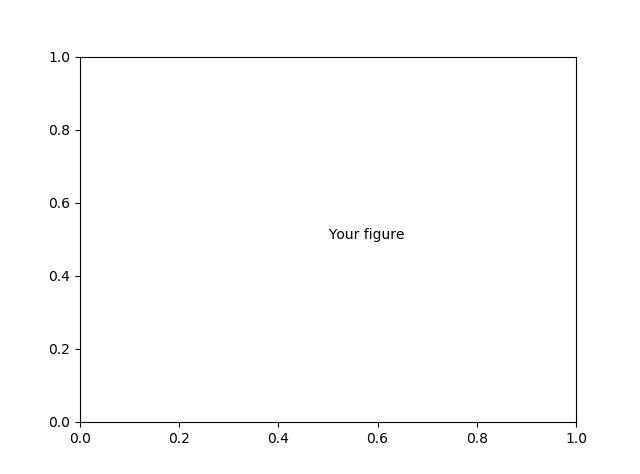
\includegraphics[width=0.45\textwidth]{./figures/empty_fig.png}
    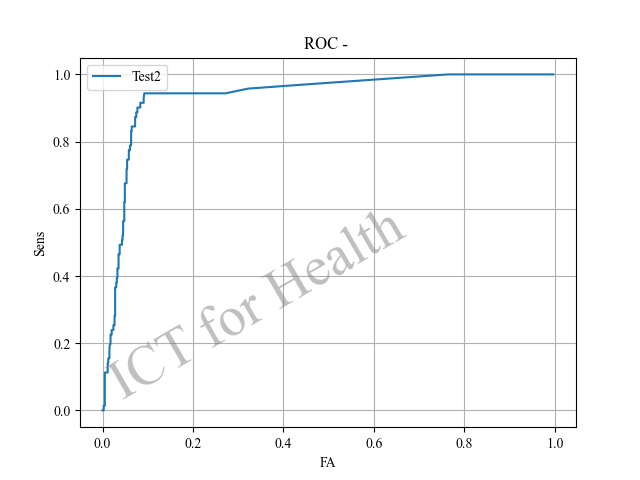
\includegraphics[width=0.45\textwidth]{./figures/Figure_ROC.png}
    \caption{ROC curve for Test 1 (left) and Test 2 (right).}
    \label{fig:ROC}
\end{figure}
For convenience, sensitivity and specificity versus threshold are also plotted in Fig. \ref{fig:sens_spec_thresh}.

\begin{figure}[ht]
    \centering
    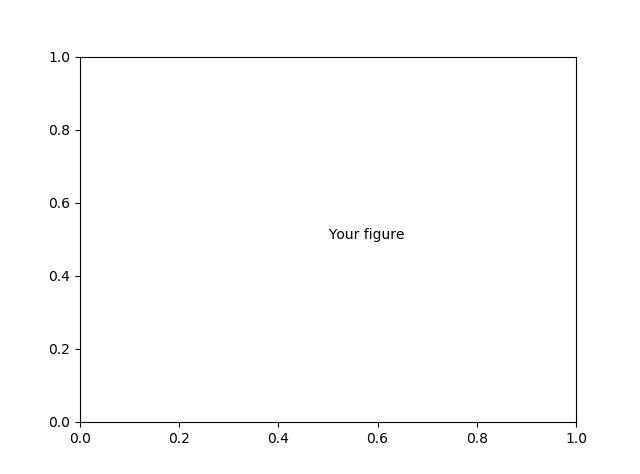
\includegraphics[width=0.45\textwidth]{./figures/empty_fig.png}
    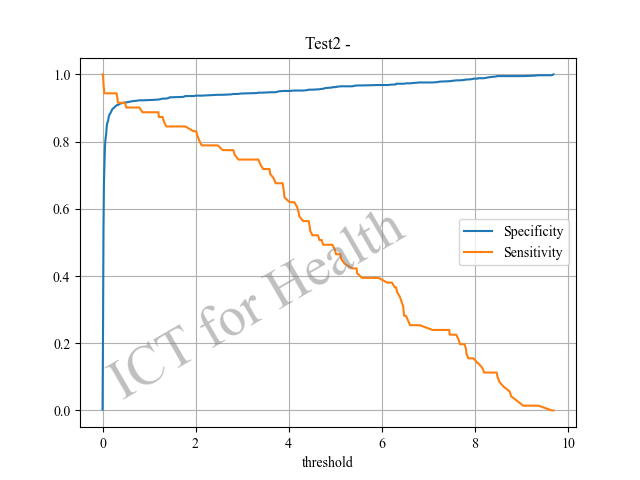
\includegraphics[width=0.45\textwidth]{./figures/Figure_sens_spec_thresh.png}
    \caption{Sensitivity and specificity versus threshold for Test 1 (left) and Test 2 (right).}
    \label{fig:sens_spec_thresh}
\end{figure}

The following notation will be used: $D$ means that the patient is really infected, $H$ means that the patient is healthy, $T_p$ means that the test is positive, $T_n$ mean that te test is negative.

The general approach in case of a positive serological test is to check again the person using the nasopharyngeal swab. This makes acceptable a  relatively large false positive probability $P(T_p|H)$, with the only drawback that healthy people stay for a couple of days at home, maybe in an anxious state. 

What cannot be accepted is instead a large false negative probability: in this case nasopharygeal swab is not tested, and the person can spread the virus to many others. Thus, it is important to have a large sensitivity $P(T_p|D)$ (probability that the test is positive given that the person has the disease), but even more important is the probability $P(D|T_n)$ that the person has the disease given the test is negative. This last probability should be kept as small as possible. 

Having assumed COVID-19 prevalence equal to 2 \%, Figs. \ref{fig:probs1} and \ref{fig:probs2} respectively show versus the threshold: 
\begin{enumerate}
    \item The probability $P(D|T_p)$ that the patient is truly infected given that the test is positive and the probability $P(D|T_n)$ that the patient is infected given that the test is negative.
    \item The probability $P(H|T_p)$ that the patient is healthy given that the test is positive and the probability $P(H|T_n)$ that the patient is healthy given that the test is negative.
\end{enumerate}

\begin{figure}
    \centering
    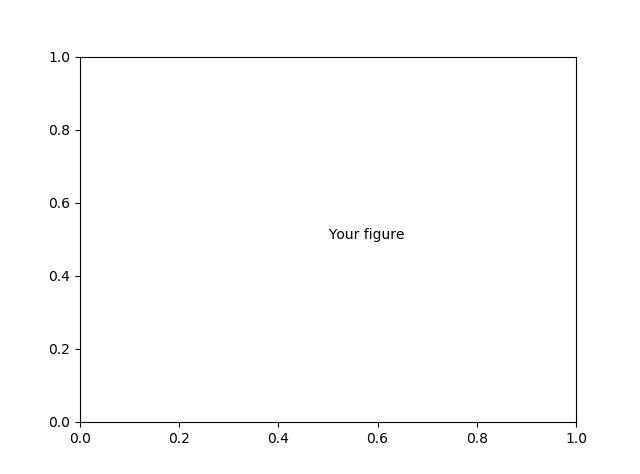
\includegraphics[width=0.45\textwidth]{./figures/empty_fig.png}
    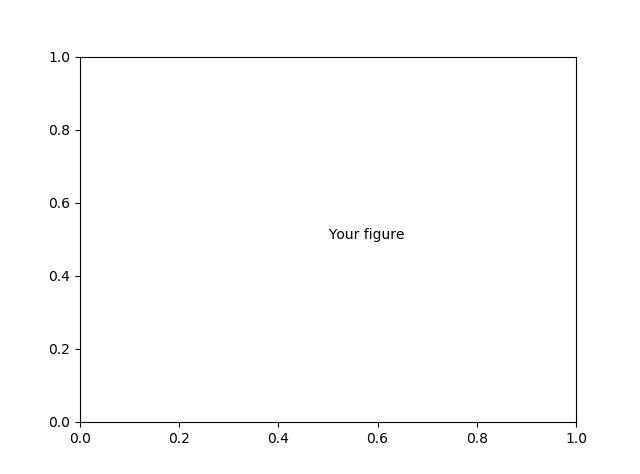
\includegraphics[width=0.45\textwidth]{./figures/empty_fig.png}
    \caption{$P(D|T_p)$ and $P(D|T_n)$ versus threshold for Test 1 (left) and Test 2 (right).}
    \label{fig:probs1}
\end{figure}
\begin{figure}
    \centering
    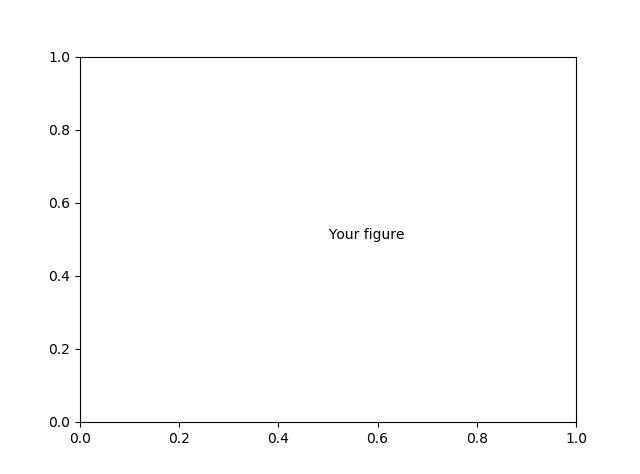
\includegraphics[width=0.45\textwidth]{./figures/empty_fig.png}
    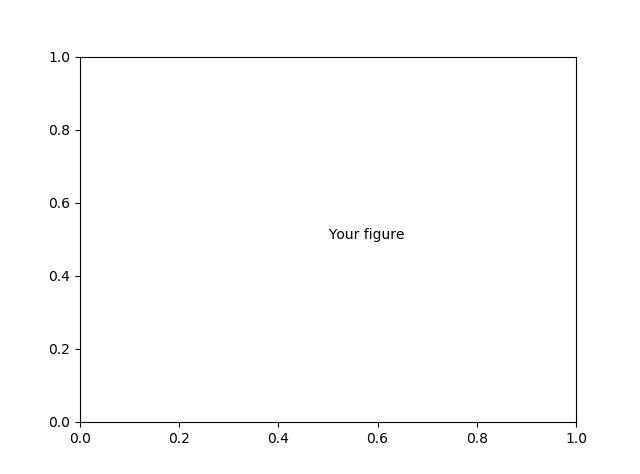
\includegraphics[width=0.45\textwidth]{./figures/empty_fig.png}
    \caption{$P(H|T_p)$ and $P(H|T_n)$ versus threshold for Test 1 (left) and Test 2 (right).}
    \label{fig:probs2}
\end{figure}

\clearpage

\section{Choice of the threshold}

\subsection{Test 1}
\begin{itemize}
    \item Sensitivity and specificity are both equal to \hl{...} when the threshold is equal to \hl{...}, in which case \hl{$P(D|T_n)= \ldots$} and  \hl{$P(D|T_p)= \ldots$}.
    \item Being this sensitivity not large enough, it is convenient to decrease the threshold; we suggest a threshold equal to \hl{...} for which:
    \begin{itemize}
        \item Sensitivity \hl{$P(T_p|D)=\ldots$}, false negative probability \hl{$P(T_n|D)=\ldots$}.
        \item Specificity \hl{$P(T_n|H)=\ldots$}, false positive probability \hl{$P(T_p|H)=\ldots$}.
        \item \hl{$P(D|T_n)=\ldots$}, \hl{$P(H|T_n)=\ldots$}.
        \item \hl{$P(D|T_p)=\ldots$}, \hl{$P(H|T_p)=\ldots$}.
    \end{itemize}
\end{itemize}

\subsection{Test 2}
\begin{itemize}
    \item Sensitivity and specificity are both equal to \hl{...} when the threshold is equal to \hl{...}, in which case \hl{$P(D|T_n)= \ldots$} and  \hl{$P(D|T_p)= \ldots$}.
    \item Since this sensitivity cannot be considered sufficient, the lower threshold  \hl{...} is recommended, for which:
    \begin{itemize}
        \item Sensitivity \hl{$P(T_p|D)=\ldots$}, false negative probability \hl{$P(T_n|D)=\ldots$}.
        \item Specificity \hl{$P(T_n|H)=\ldots$}, false positive probability \hl{$P(T_p|H)=\ldots$}.
        \item \hl{$P(D|T_n)=\ldots$}, \hl{$P(H|T_n)=\ldots$}.
        \item \hl{$P(D|T_p)=\ldots$}, \hl{$P(H|T_p)=\ldots$}.
    \end{itemize}
\end{itemize}
\section{Conclusions}
\hl{.....}

 


\begin{thebibliography}{9}
\bibitem{DBSCAN} Ester M., Kriegel H-P., Sander J., Xu X.  \textit{A density-based algorithm for discovering clusters in large spatial databases with noise}. Proceedings of the Second International Conference on Knowledge Discovery and Data Mining 1996 (KDD-96), pp. 226-231. AAAI Press. 
\end{thebibliography}

\end{document}
